\documentclass{../template/texnote}


\title{\textbf{\capitalisewords{Exploring the Explosive Side of the Sun}}}
\begin{document}
    \maketitle \currentdoc{note}
    %<*note>

% \begin{figure}
%     \centering
%     
\includegraphics[scale=0.55]{Linn/WByS0gCAwV_20190711111040412.jpg}
%     \label{fig:green}
% \end{figure}

\section{The Sun and Life on Earth}
Energy is a fundamental requirement for life. The most common characteristics of life, namely, organization, metabolism, response to stimuli, reproduction, adaptation and evolution, all require energy. All almost life forms on Earth depend on the Sun for their energy (There are organisms that can derive their energy by oxidizing inorganic compounds such as hydrogen sulfide, ammonia or methane. They are mostly found in environments without sunlight such as deep-sea hydrothermal vents, hot springs, and caves). It is no wonder then that almost of all the early civilizations and cultures worshiped the Sun as a deity. The warmth and light of the Sun was a welcome relief from the cold and dark nights that made him afraid. The Sun's regular rising and setting provided a sense of order and predictability to the natural world, which was often seen as chaotic and unpredictable. The brightness and intensity of the Sun gave it a divine glow that we have come to associate with many other deities. Without any apparent source of energy the Sun was a mystery to the ancients and this made it worthy to be worshiped by countless generations of people.

\begin{figure}
    \centering
    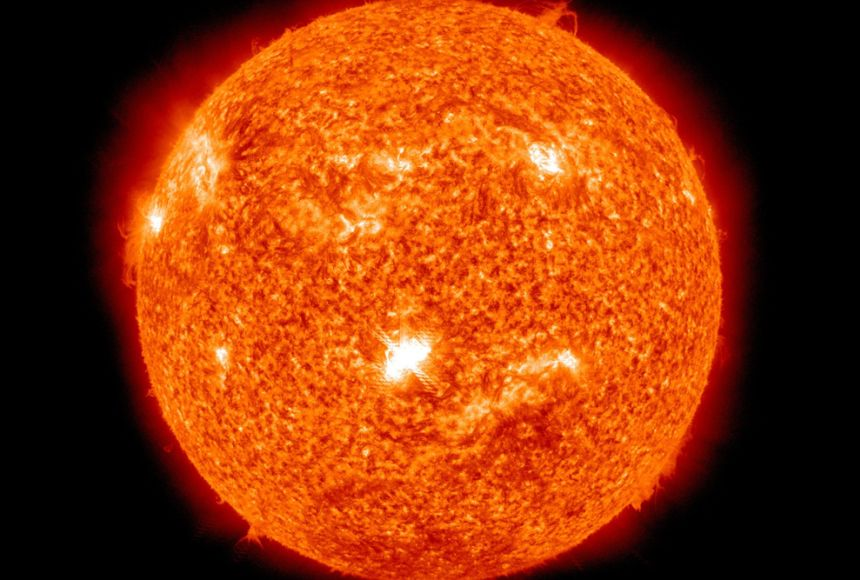
\includegraphics[scale=0.50]{Linn/sun-blasts-a-m66-flare.jpg}
    \caption{Sun Blasts a M6.6 Flare
On Feb. 13th at 1738 UT, sunspot 1158 unleashed the strongest solar flare of the year so far, an M6.6-category blast. Image Credit:  NASA/ SDO/ AIA}
    \label{fig:sun}
\end{figure}

\section{Historical Record of Solar Explosions}
Today, worshiping the Sun might sound to be a ridiculous thing to do. The scientific revolution brought about a paradigm shift in our perception of the Sun. The Italian astronomer Galileo Galilei made the first recorded observations of Sunspots. 
Galileo's observations showed that the Sun had dark spots on its surface that appeared to change in size and shape over time. These observations were groundbreaking, as they challenged the prevailing view of the Sun as a perfect, unblemished celestial body, and paved the way for further research into the Sun's physical properties and behavior. Samuel Heinrich Schwabe discovered the sunspot cycle in 1844. This is a periodic variation in the number of sunspots observed. The average period is seen to be close to 11 years with the actual period between 7 and 17 years.
The fact that there can be sudden explosions on the surface of the sun was discovered on 1 September 1859 by Richard Carrington, an English astronomer. Carrington was studying a sunspot with his telescope. As is usually the case with astronomers who study the sun, he projected an image of the sun onto a screen and observed it. He was probably surprised to find that ‘two patches of intensely bright and white light broke out’ in the middle of the sunspot.
% \begin{figure}
%     \centering
%     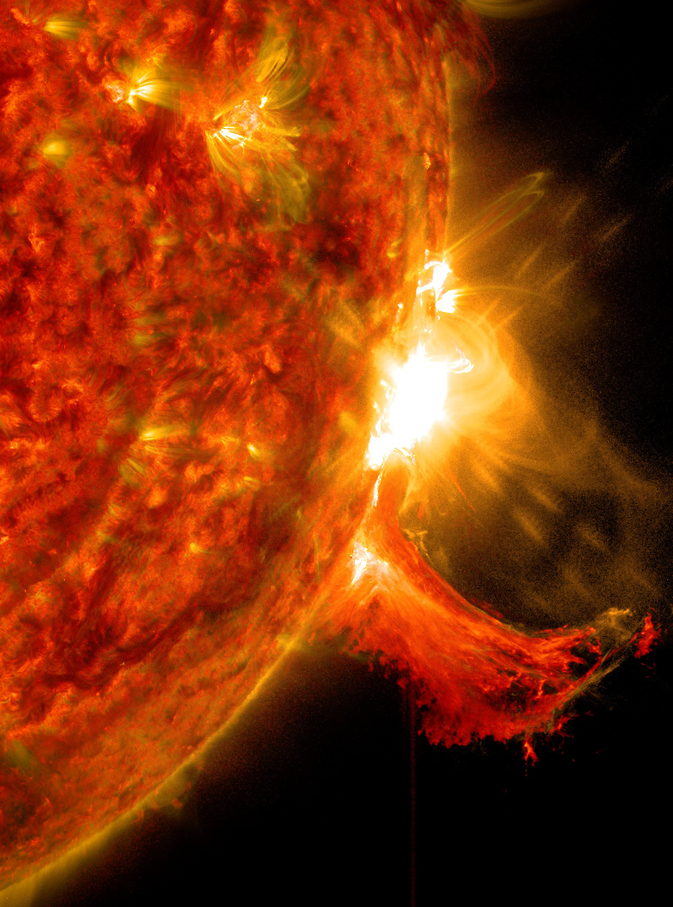
\includegraphics[scale=0.45]{Linn/m7.3-flare-zoom_0.jpg}
%     \caption{Sun Blasts a M6.6 Flare
% On Feb. 13th at 1738 UT, sunspot 1158 unleashed the strongest solar flare of the year so far, an M6.6-category blast.}
%     \label{fig:flare}
% \end{figure}

\begin{figure}
    \centering
    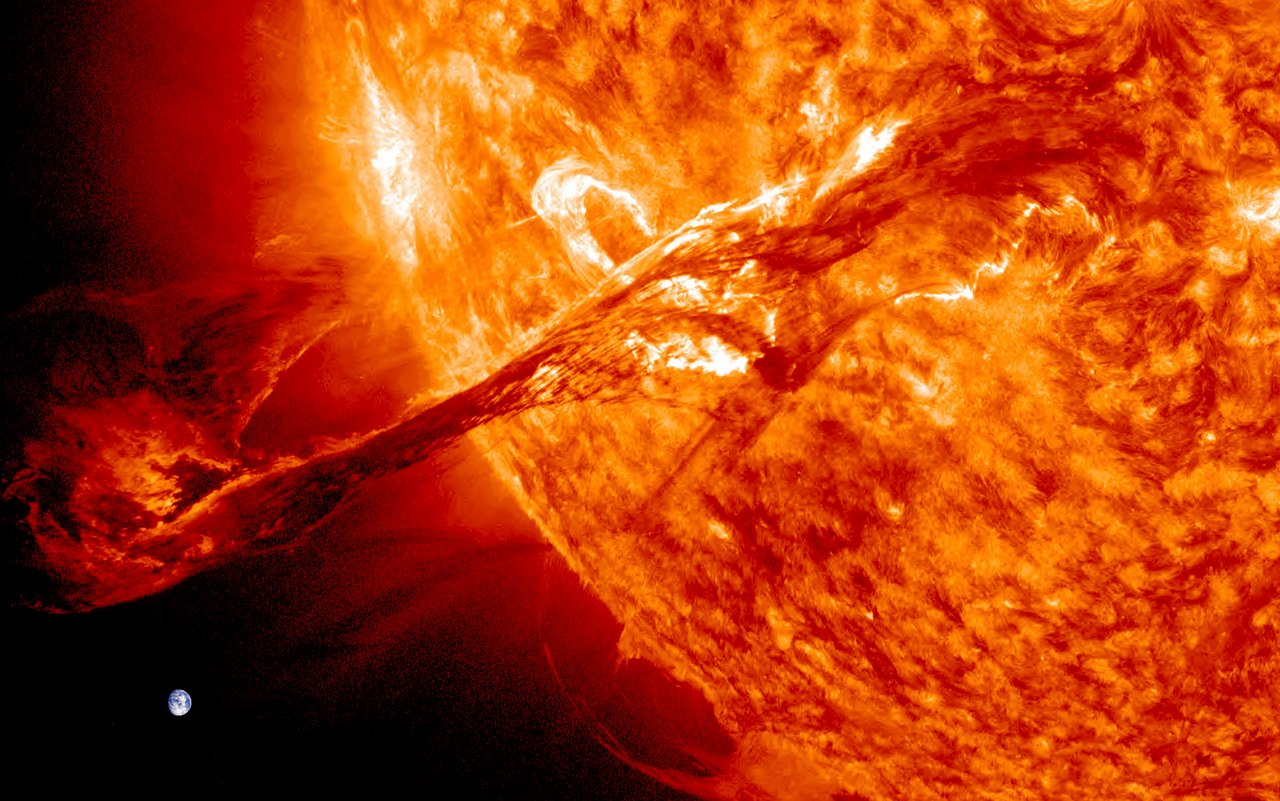
\includegraphics[scale=0.35]{Linn/0303_F_solar_flare_earth_scale.jpg}
    \caption{The Earth is dwarfed by a giant explosion on the Sun that ejects huge amounts of hot gas into space. Here the sizes of the Earth and the Sun are shown to scale, but not the distance between them. Image Credit: NASA}
    \label{fig:flare_b}
\end{figure}

\section{Do We Need to Predict These Outbursts?}
About 18 hours after he saw the flare, the magnetic observing station in Kew reported a sudden violent change in the earth’s magnetic field, known as a geomagnetic storm. The storm was so strong that it disrupted telegraph communications around the world and caused auroras to be visible at lower latitudes than usual.
One of the earliest known geomagnetic storms was the ``Bastille Day Event'' of July 14, 1770. This storm was observed by French astronomer Jean-Andre Deluc, who noted that a compass needle in his possession was behaving erratically. Other observers in Europe and North America also reported unusual auroras and magnetic disturbances around the same time.
Carrington made the first indirect suggestion made by anybody that an explosion in the sun could cause abnormal things to happen on the Earth. He made this observation at the meeting of the Royal Astronomical Society about two months after the discovery. 
Several other solar storms have been observed ever since. The greatest solar storm of the Space Age was observed in 1989 which led to a blackout in the Canadian province of Quebec due to the outage of their power grid. Interestingly, the first flare recorded by any human being (dubbed ``The Carrington Event'') is also the strongest flare ever to have been observed.
The evidence for this was unearthed by researchers who found measurements of the storm as far away from the geomagnetic poles as India. This flare must have been at least three times as strong as the 1989 flare that caused havoc in Quebec. 
\section{How the Modern World is Becoming More Vulnerable to Solar Flares?}


The fact that the Carrington event was not recorded as a catastrophic event in history whereas the Quebec solar flare made major headlines shows how the world has become increasingly dependent on technology. Not just any technology but technology that is vulnerable to solar flares. The connection between solar flares and modern technology can be understood with Michael Faraday's observation of magnetic fields inducing electric currents. 
Our current understanding of the sun shows that it must be a ball of hot burning gas. But the gas is mostly in the inner layers, whereas the outer layers exists as plasma due to the very high temperatures. In 1958 Eugene Parker proposed the theory of the Solar Wind where he found that the high temperature of the corona should cause a continuous wind of gas and plasma to blow through the entire solar system. Solar flares cause a sudden increase in the influx of these particles. 
The earth’s magnetic field mitigate the effects of sudden solar disturbances to some extent. However this protective shield is weakest near the geomagnetic poles because of a lower density of magnetic field lines. The polar auroras are a harmless consequence of this fact. 
One geomagnetic pole is located in the Canadian Arctic. This explains why the major blackout occurred in the Canadian province of Quebec. The interaction of the electrical charged particles with the Earth's magnetic field is capable of causing induced currents in our electrical grids and subsequently cause them to fail.
There are several other ways in which solar flares affect our lives. Radio communications are an essential part of modern technologies. The ionosphere is what makes radio communications to distant places on the Earth possible which would otherwise be impossible due to the Earth's curvature. Solar flares disturb the ionosphere and thus cause disturbances in radio communication. The north geomagnetic pole is a frequent route for passengers between Europe and North America. After a major solar flare, airline companies would have to reroute flights else the pilots lose radio contact with ground stations. 
Artificial satellites are another piece of technology that has become ubiquitous to life on Earth. We rely on them for everything from television broadcasting to daily navigation (GPS satellites). A major solar flare can roast the electronics on board if precautions are not put in place.
All this points to an increased need to understand the dynamics of our Sun. Knowing more about the solar activity and sunspots are critical. Advance warning of the solar flare predictions are important for disaster mitigation. 

\begin{figure}
    \centering
    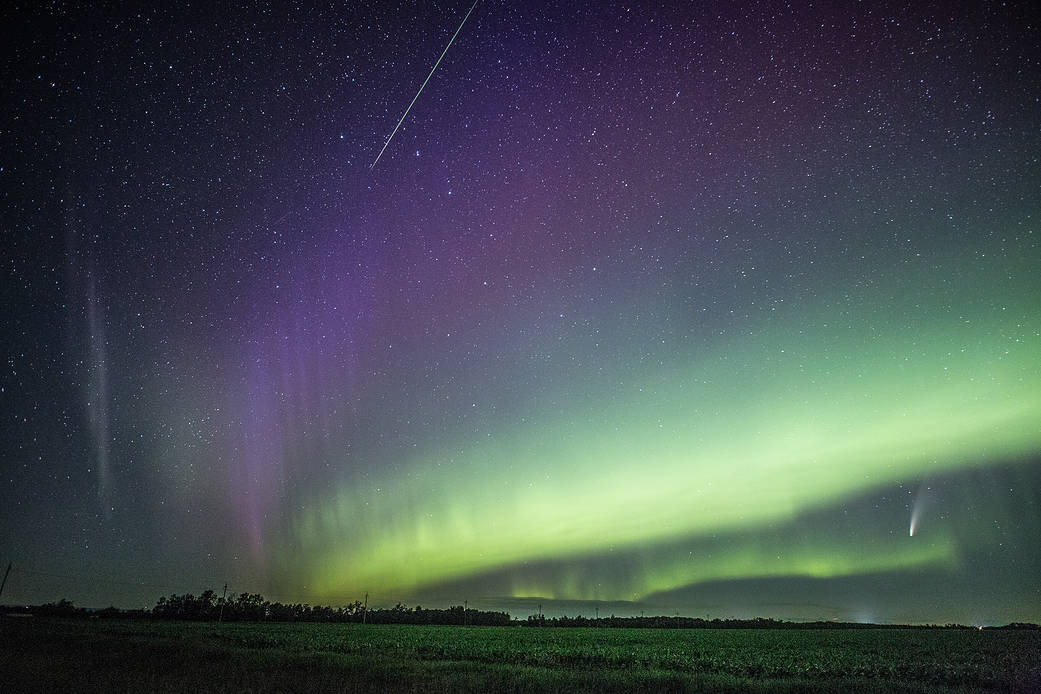
\includegraphics[scale=0.45]{Linn/9744_steve_neowise_aurora_meteor_donna_lach-sm.jpg}
    \caption{Comet NEOWISE is visible in an aurora-filled sky in this photo taken on July 14, 2020, by Aurorasaurus Ambassador Donna Lach. Image Credit: NASA}
    \label{fig:aurora}
\end{figure}


\section{References}
\begin{enumerate}

 \item Choudhuri, Arnab Rai. Nature's Third Cycle: A Story of Sunspots. Oxford; New York: Oxford University Press, 2015.
 \item Karttunen, Hannu, Pekka Kröger, Heikki Oja, Markku Poutanen, and Karl Johan Donner, eds. Fundamental Astronomy. Berlin, Heidelberg: Springer Berlin Heidelberg, 2017. https://doi.org/10.1007/978-3-662-53045-0.
    \item \href{https://universemagazine.com/en/did-you-know-that-12-interesting-facts-about-the-sun/}{Did you know that? 12 interesting facts about the Sun.}
    \item \href{https://en.wikipedia.org/wiki/List_of_solar_storms}{List of solar storms}
\end{enumerate}
    %</note>
    \printbibliography
\end{document}
